%-----------------------------------------------------------------------------%
\chapter{\babDua}
\label{bab:2}
%-----------------------------------------------------------------------------%
This chapter displays the results of the literature study that has been done to help further the research. The literature study is based on relevant topics that are used in this research.


%-----------------------------------------------------------------------------%
\section{Kubernetes}
\label{sec:kubernetes}
Kubernetes is used to manage, monitor, and scale containers of a cluster and can be extended to geo-distributed clusters when hosted on a cloud platform. At first, application deployment is done by hosting the application on a dedicated machine on-premise. This changed when Cloud providers were introduced, where Cloud-based services helped improve deployment management through monitoring and scalability through cloud servers, removing the need of maintaining a physical server. The deployment process itself did not change much until a breakthrough in the form of Docker containers was introduced in 2010. 

Docker utilizes virtual machines that offer consistency and reliability, regardless of which machine it's being hosted on. This means that application behavior is consistent regardless of the machine itself as long as it is capable of running Docker. Docker's containerization solution, however, is limited to a single application. In reality, a complete application consists of multiple layers, for example, a three-tier application consisting of a frontend, backend, and database layer. In this case, Kubernetes extends Docker's containerization solution to a complete and production-ready application by managing containers and enabling them to communicate with each other.

Additionally, containers are deployed as Pods, the smallest unit of a Kubernetes resource. Furthermore, a higher level Service resource is used to group Pods, manage their lifecycle, and create replicas of them. \citep{jeffery-2021}. This is proven to be an extremely useful feature, as the Service resource can be grouped by unique identifiers such as service name and namespace, which can be used to deploy multiple Service resources inside multiple clusters. This is the main idea of geo-distributed clusters, where Kubernetes services are interconnected through clusters which has benefits such as geo-aware routing and additional reliability measures through cluster failover, which we will discuss in the next section.


% Kubernetes has changed application deployment by offering a 

\section{Geo-distributed Clusters}
\label{sec:geo-distirbutedCluster}
% The recent trend is to use traditional cloud resources in conjunction with ever-increasing edge/fog computing resources located at the network edges. Their exploitation allows us to decentralize the execution of applications, by moving the computation closer to data sources and consumers,
The full capabilities of a Kubernetes application are put on display with the help of cloud providers. By using traditional cloud resources in conjunction with edge/fog computing resources located at the network edges, application execution can be done closer to data sources and consumers, thus increasing the scalability of applications and decreasing their response time \citep{rossi-2020}. Cloud providers such as Google Cloud, Amazon Web Services, and Azure, all have servers available in different areas of the globe, making them a great candidate for the adoption of this application architecture. By utilizing the wide coverage of cloud servers, an application can be deployed to every available region to cater to the users of each region without the need of having an on-premise self-hosted physical server. This can be seen in \autoref{fig:geo-diagram}, where this approach provides a better server coverage than just a centralized deployment.

\begin{figure}
	\centering
	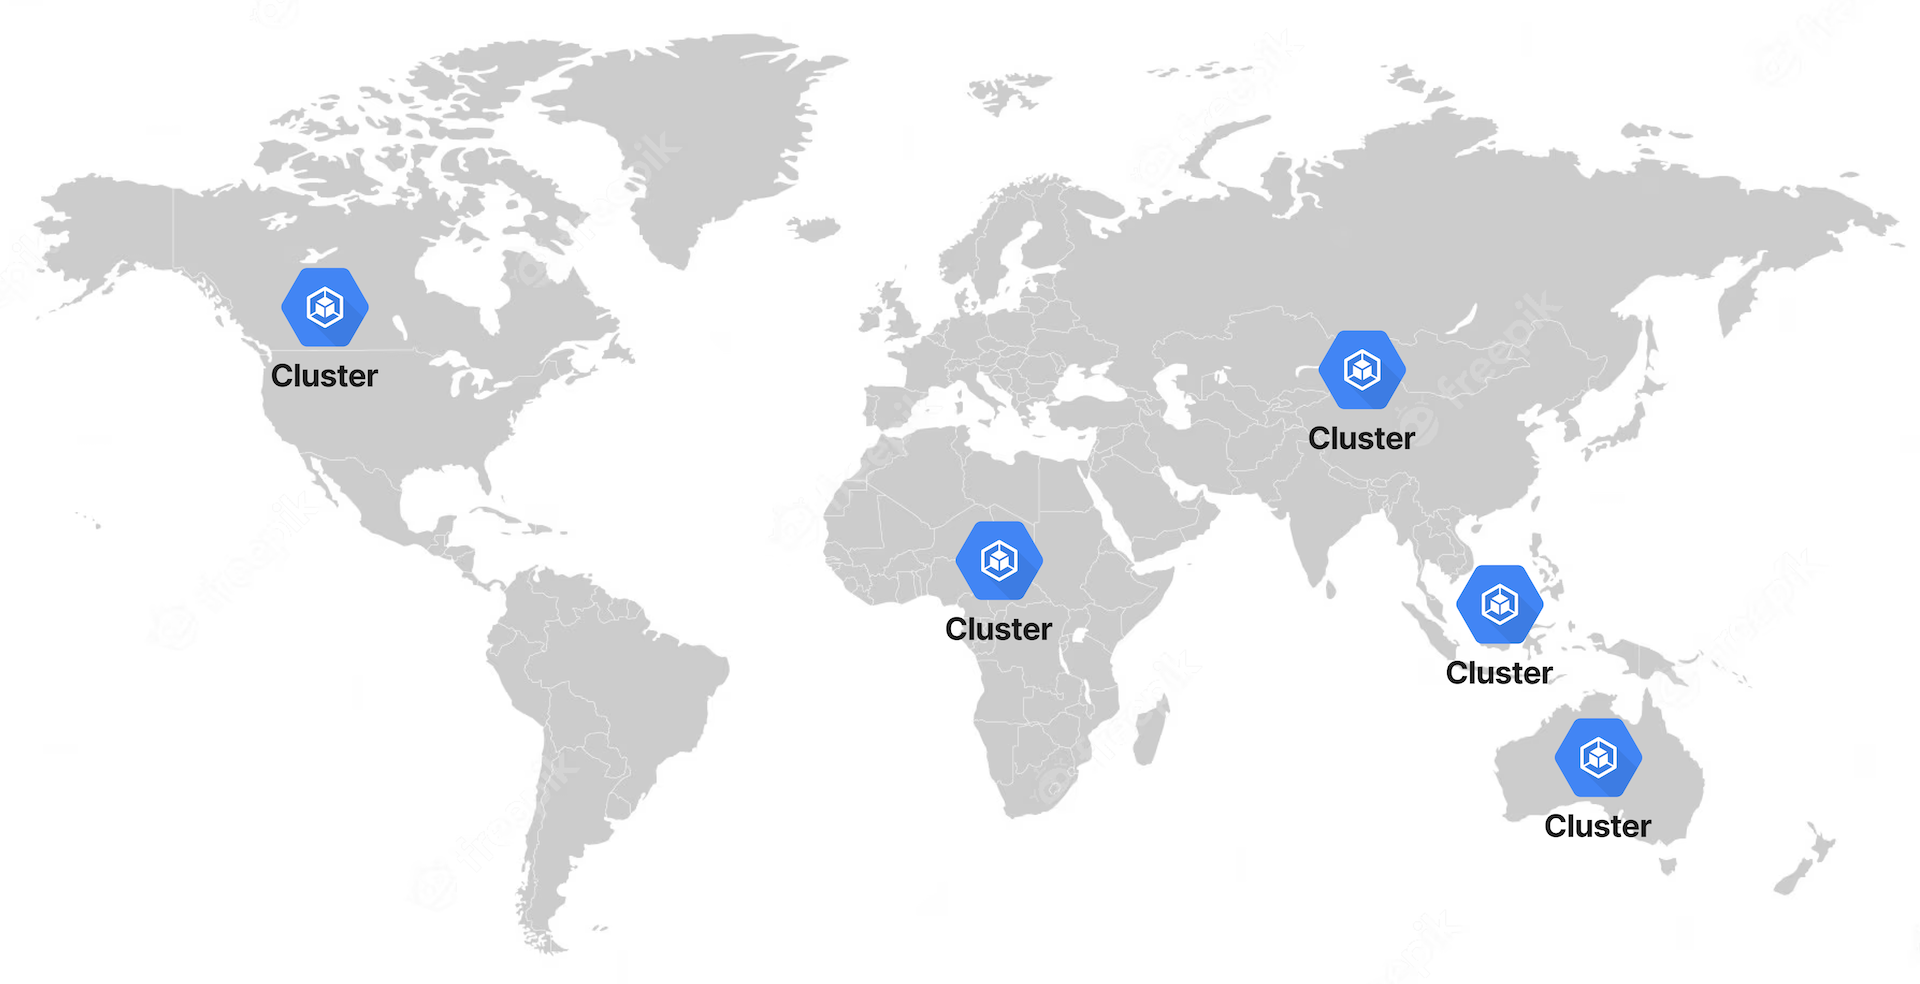
\includegraphics[width=1\textwidth]{assets/diagrams/geo-diagram.png}
	\caption{Geographically distributed clusters in different areas of the world.}
	\label{fig:geo-diagram}
\end{figure}

Geo-distributed clusters are multiple clusters hosted in different areas of the region. When an application's user base grows and spreads globally, a single central deployment may not offer the best user experience. The physical distance of a user to the server matters, which makes geo-distributed application deployment a good solution to accommodate users from all over the world. With the help of Kubernetes and a cloud provider, multi-regional deployment has never been easier. It is, however, a relatively new area in software development, and not much has been studied about the different approaches of this architecture. For this research, we have chosen two approaches: MultiClusterService with MultiClusterIngress and Istio / Anthos Service Mesh, as they are both are supported on the Google Cloud Platform.

In addition, geo-distributed clusters can be extended to databases, which can be seen in implementations such as CocroachDB. As different countries have different regulations, it is becoming a necessity for multinational companies to store user data in their respective region in order to comply with regulations. Data should be stored close to the users who access it most frequently and follow them when they travel to prevent high latencies caused by long-distance data retrieval \citep{taft-2020}. We used a simpler approach to achieve database geo-awareness, however, as geo-distributed databases introduce added complexities such as partition and replication, which are outside of this research scope.
% In addition, geo-distributed clusters can be extended to databases, which can be seen in implementations such as CocroachDB. The same benefits such as reduced latency can be gained in the data layer of an application, as different regulations between countries 


% Two geo-distributed clusters approaches studied in this research are MultiClusterService with MultiClusterIngress and Istio / Anthos Service Mesh.

\section{MultiClusterService (MCS) with MultiClusterIngress (MCI) (MCS with MCI}
To connect identical services across geo-distributed clusters, Fleet, MultiClusterIngresss, and MultiClusterService must be configured. A Fleet is a group of clusters that are visible to the MultiClusterIngress and can be used as backends. Inside a Fleet, a cluster needs to be designated as a config cluster where MultiClusterIngress and MultiClusterService are configured and deployed. Clusters that are registered to a Fleet besides the config cluster are called member clusters. 

MultiClusterService (MCS) is a custom GKE resource that allows services with the same selectors to be considered the same by creating derived services in the member clusters. The derived service creates a Network Endpoint Group (NEG) in every target cluster which tracks pod endpoints and allows service discovery, as shown in \autoref{fig:mcs-derivation}. MCS integrates with Google's Fleet to define target clusters to create derived service resources. By default, every cluster registered to a Fleet is considered a target cluster.

MultiClusterIngress (MCI) is a custom resource that sends traffic to the default backend MCS or based on rules configured to route hosts to a certain backend MCS and creates a layer 7 Virtual IP (VIP) address that routes traffic to backends that are configured in multiple clusters as MCS and can be accessed by public users. MultiClusterService and MultiClusterIngress are configured identically to their non-multi counterpart and are only deployed in the config cluster.

\begin{figure}
	\centering
	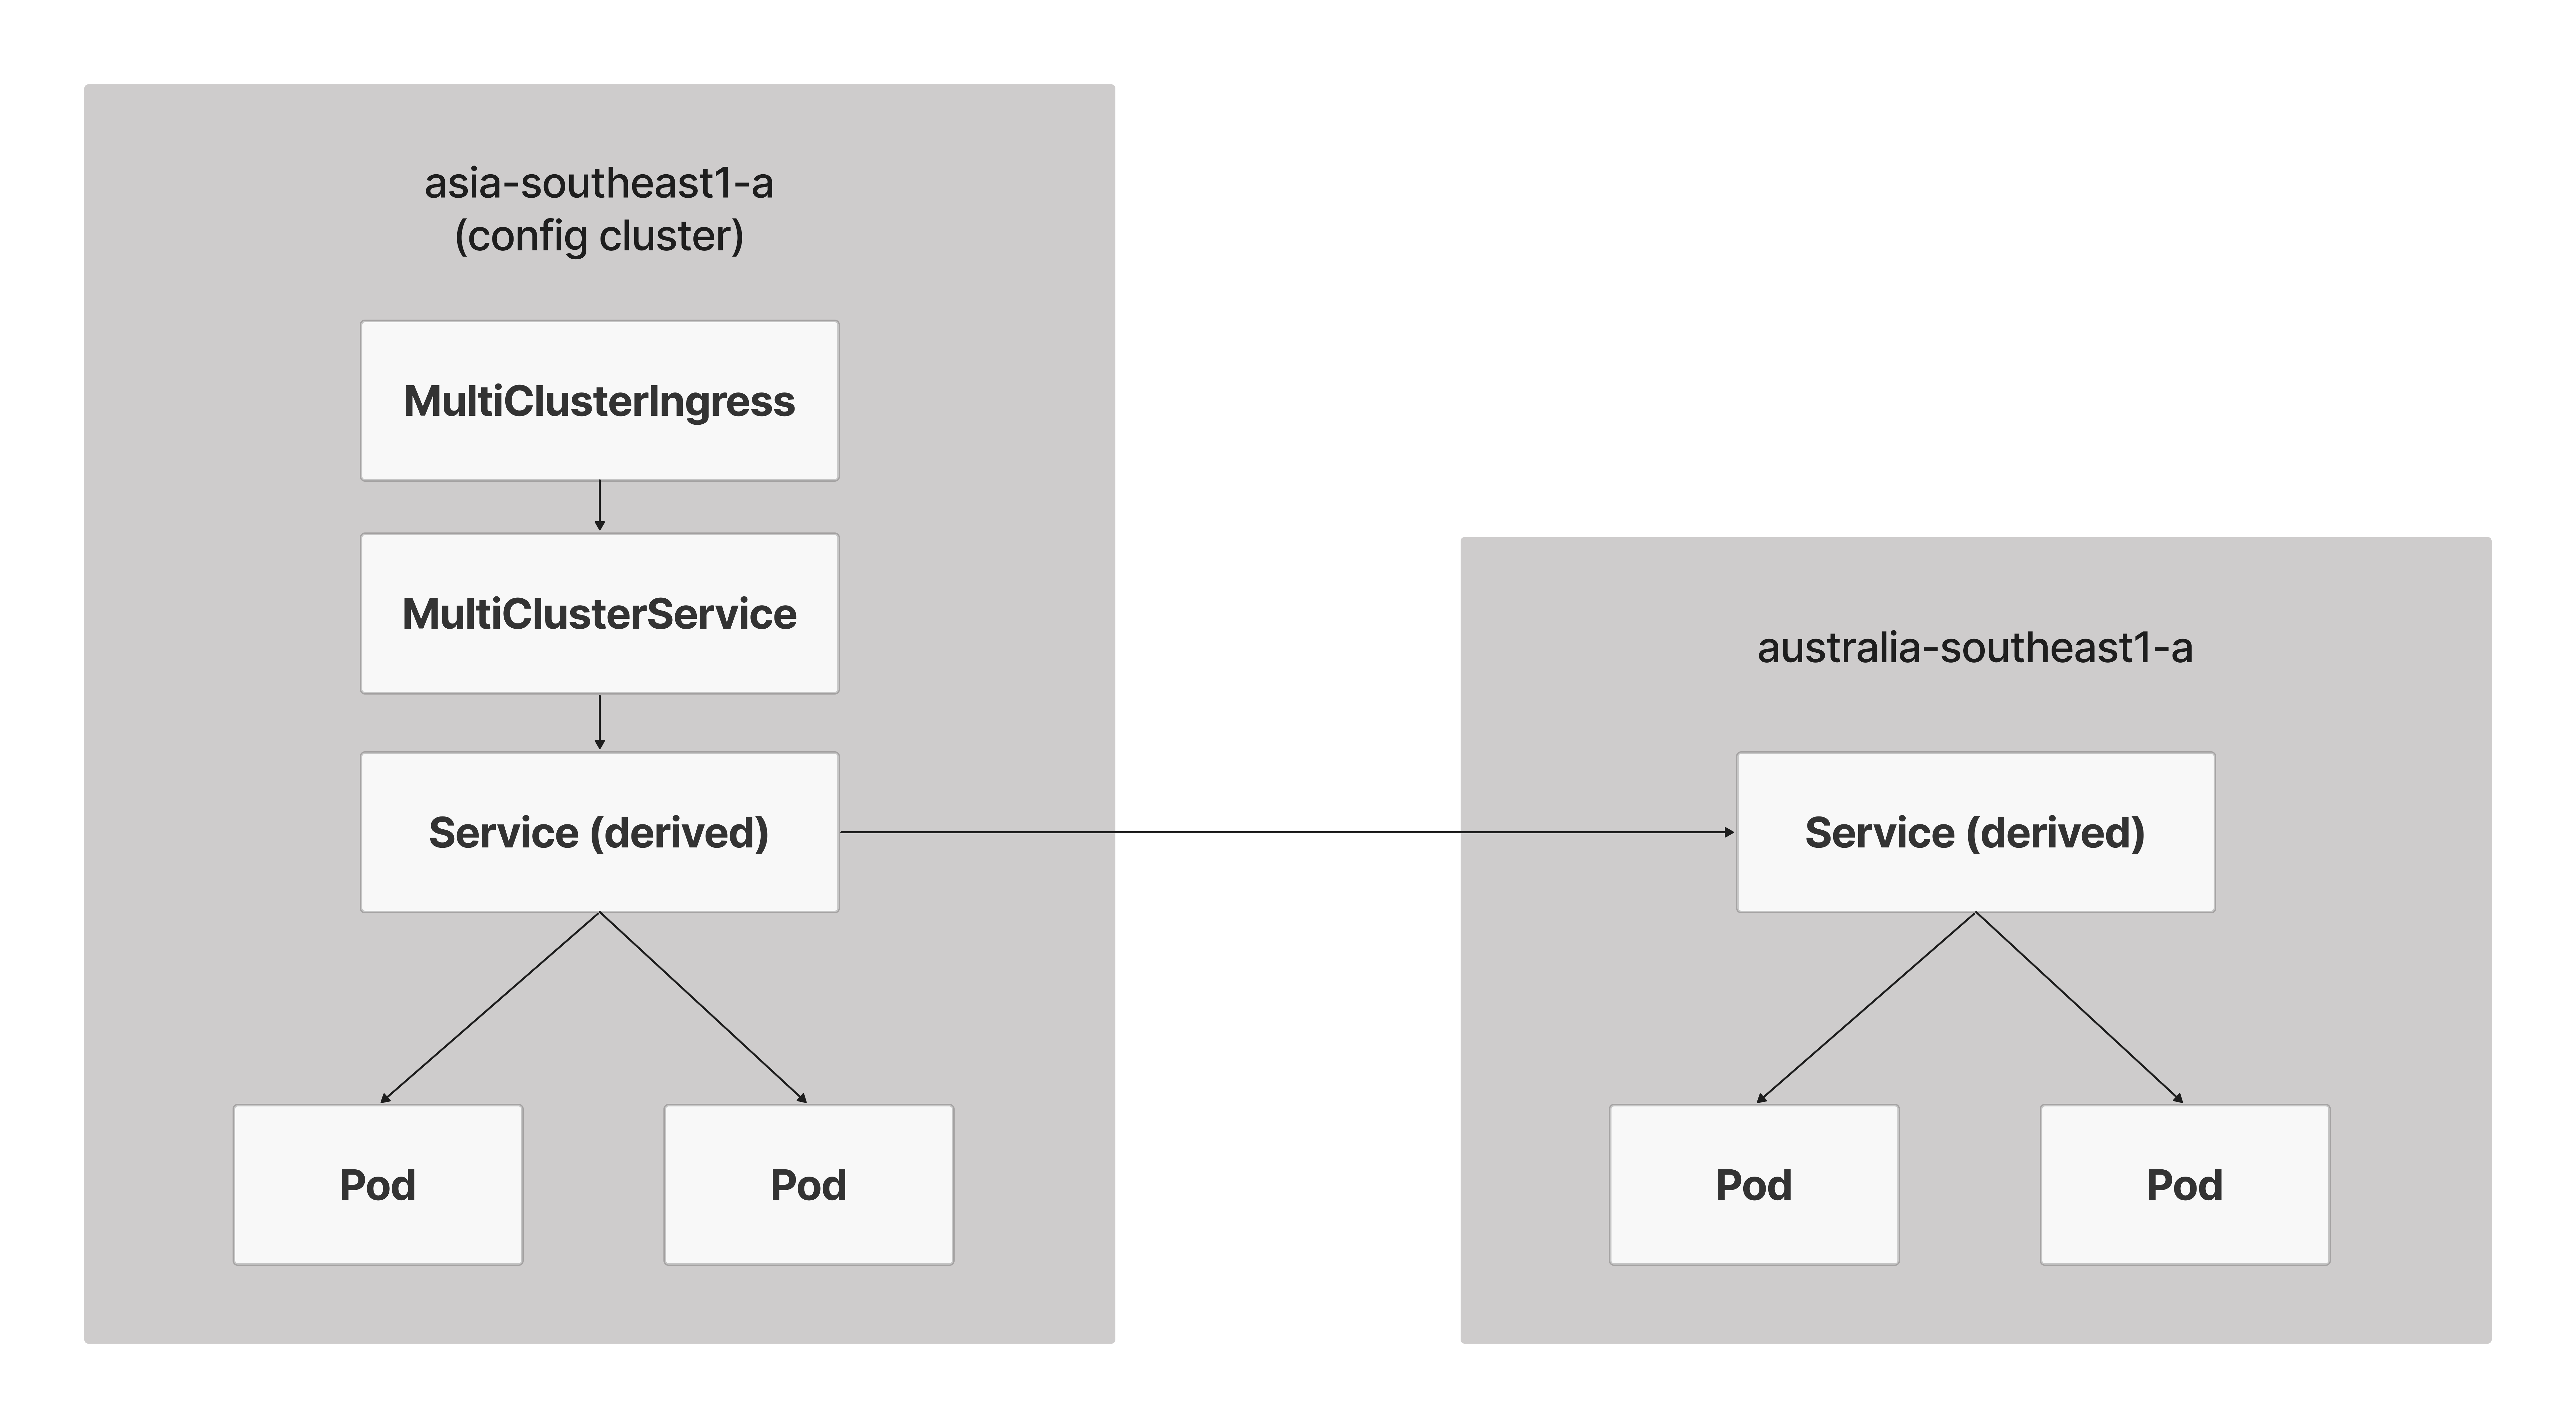
\includegraphics[width=1\textwidth]{assets/diagrams/mcs-mci.png}
	\caption{Service derivation using MultiClusterIngress and MultiClusterService.}
	\label{fig:mcs-derivation}
\end{figure}

% \section{Google Cloud Load Balancer}
% \label{sec:cloudLoadBalancer}
In a multi-cluster GKE setup using MCS with MCI, MCI deploys load balancers across clusters registered to a Fleet. The type of load balancer deployed by an MCI is a global external load balancer and is categorized as north-south routing, meaning that it routes traffic from outside to inside of the data center, as seen in \autoref{fig:gclb-diagram}.

\begin{figure}
	\centering
	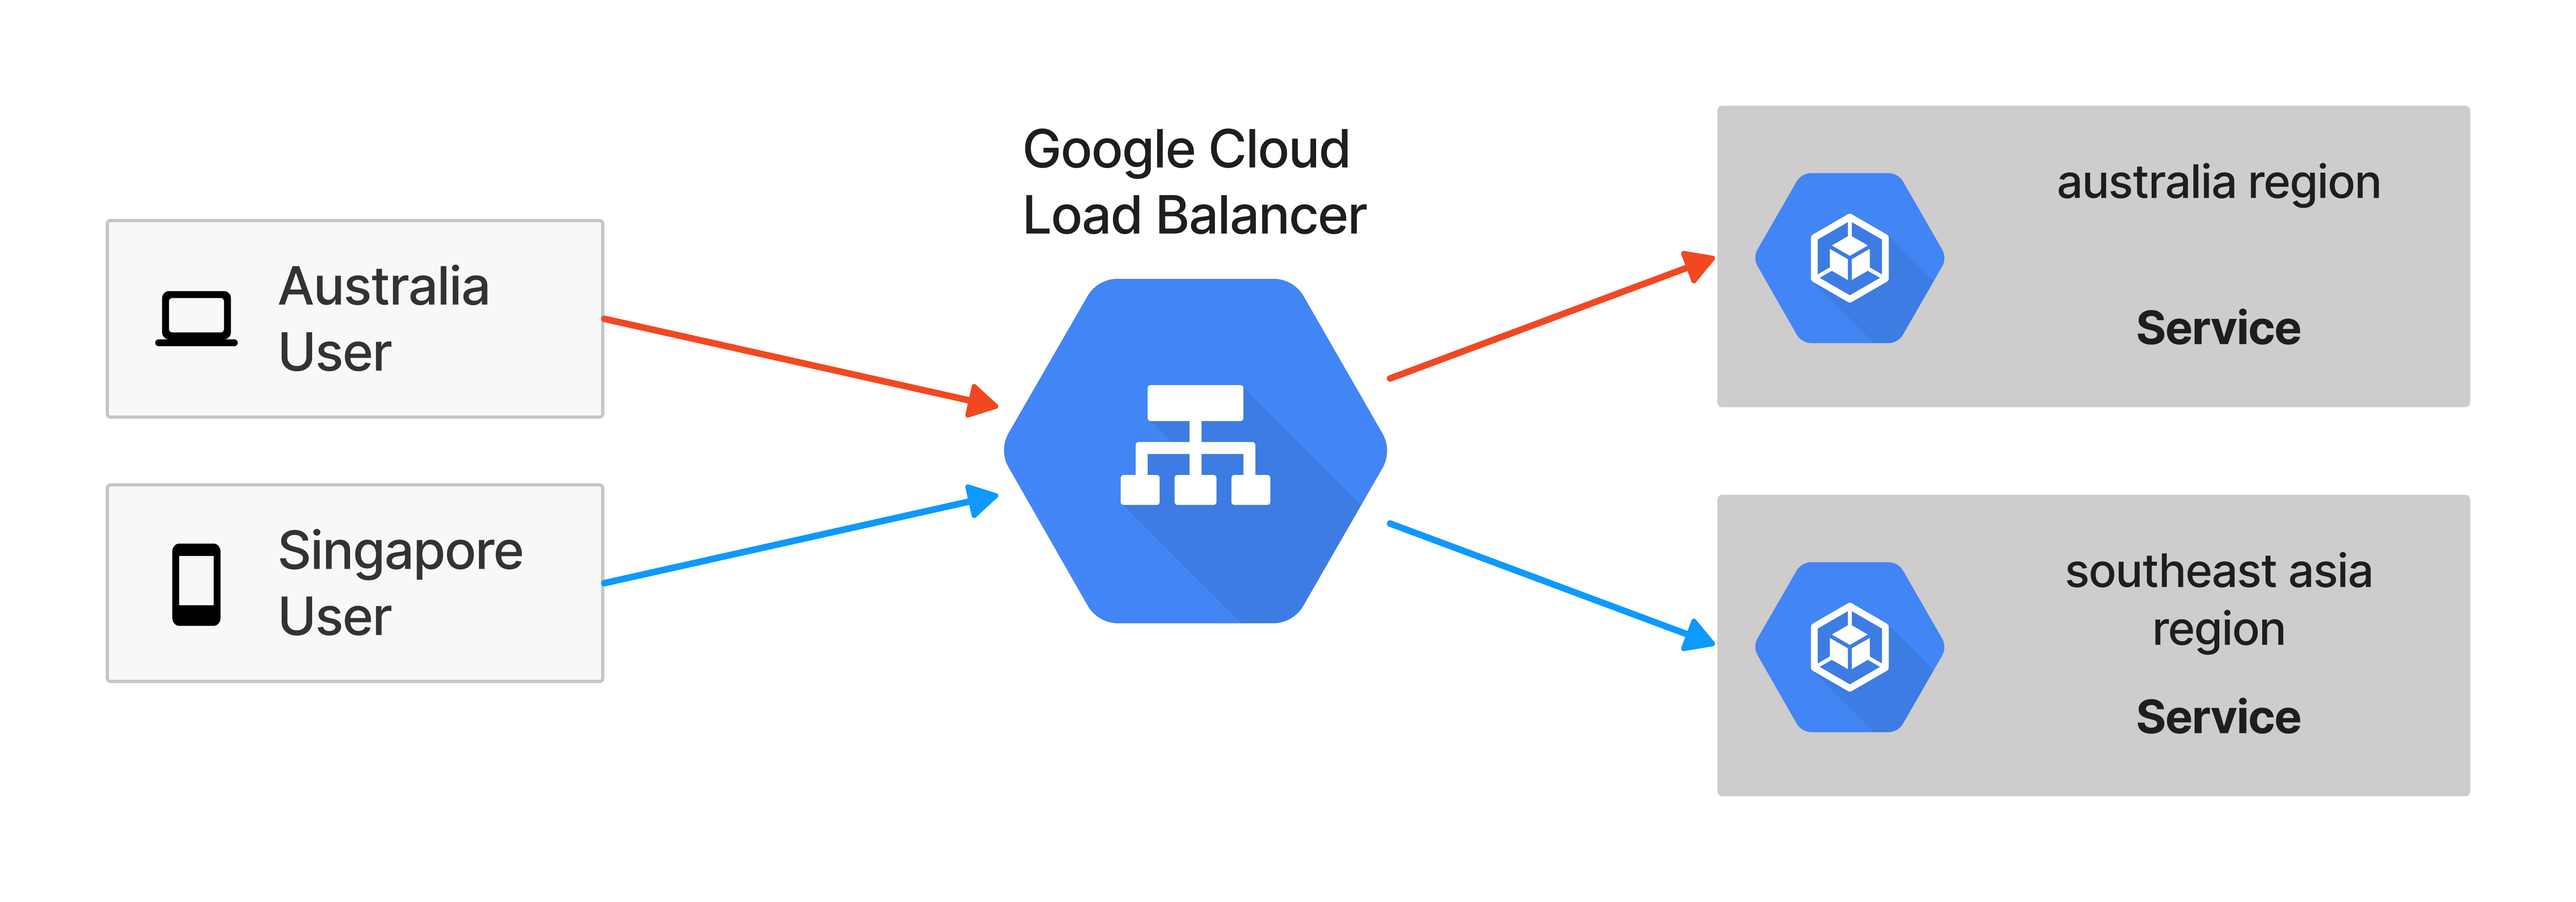
\includegraphics[width=1\textwidth]{assets/diagrams/gclb-diagram.png}
	\caption{Google Cloud Load Balancer traffic routing.}
	\label{fig:gclb-diagram}
\end{figure}

The global external load balancer routes traffic to the closest Google Point of Presence (PoP) and uses a single anycast IP address deployed to multiple regions \citep{google-mci-2023}. There is also a premium network tier that offers cold-potato routing to Google PoPs and hot-potato routing inside Google networks.
% Google Cloud Load Balancer uses a single Anycast IP which routes users to the closest Google Point of Presence (PoP).

\section{Istio / Anthos Service Mesh}
\label{sec:istio}
The other option for multi-cluster Kubernetes deployment presented in this research is using Istio / Anthos Service Mesh. Istio is an open-sourced service mesh platform that is used to connect microservices and adds features such as observability, security, and traffic management. Istio on GKE is not supported since September 2022 but users can still use Istio under the name of Anthos Service Mesh on the Google Cloud Platform. Anthos Service Mesh (ASM) is compatible with Istio custom resources. ASM has the benefit of a managed control plane that handles automatic upgrades as well as a managed data plane that automatically upgrades sidecar proxies and injected gateways by evicting old pods that are running a prior version \citep{google-asm-2023}. Automatic sidecar injection is the core of Istio's functionality, allowing pods to be injected with the Envoy proxy at creation, as shown in \autoref{fig:envoy-proxy-injection}. Envoy proxy mediates all inbound and outbound traffic for all services in a service mesh. For a multi-cluster Anthos Service Mesh, ASM integrates with the Fleet API just like the MCS with MCI approach, but there is no config cluster. Instead, installing ASM on every cluster is needed to register them to the service mesh.

\begin{figure}
	\centering
	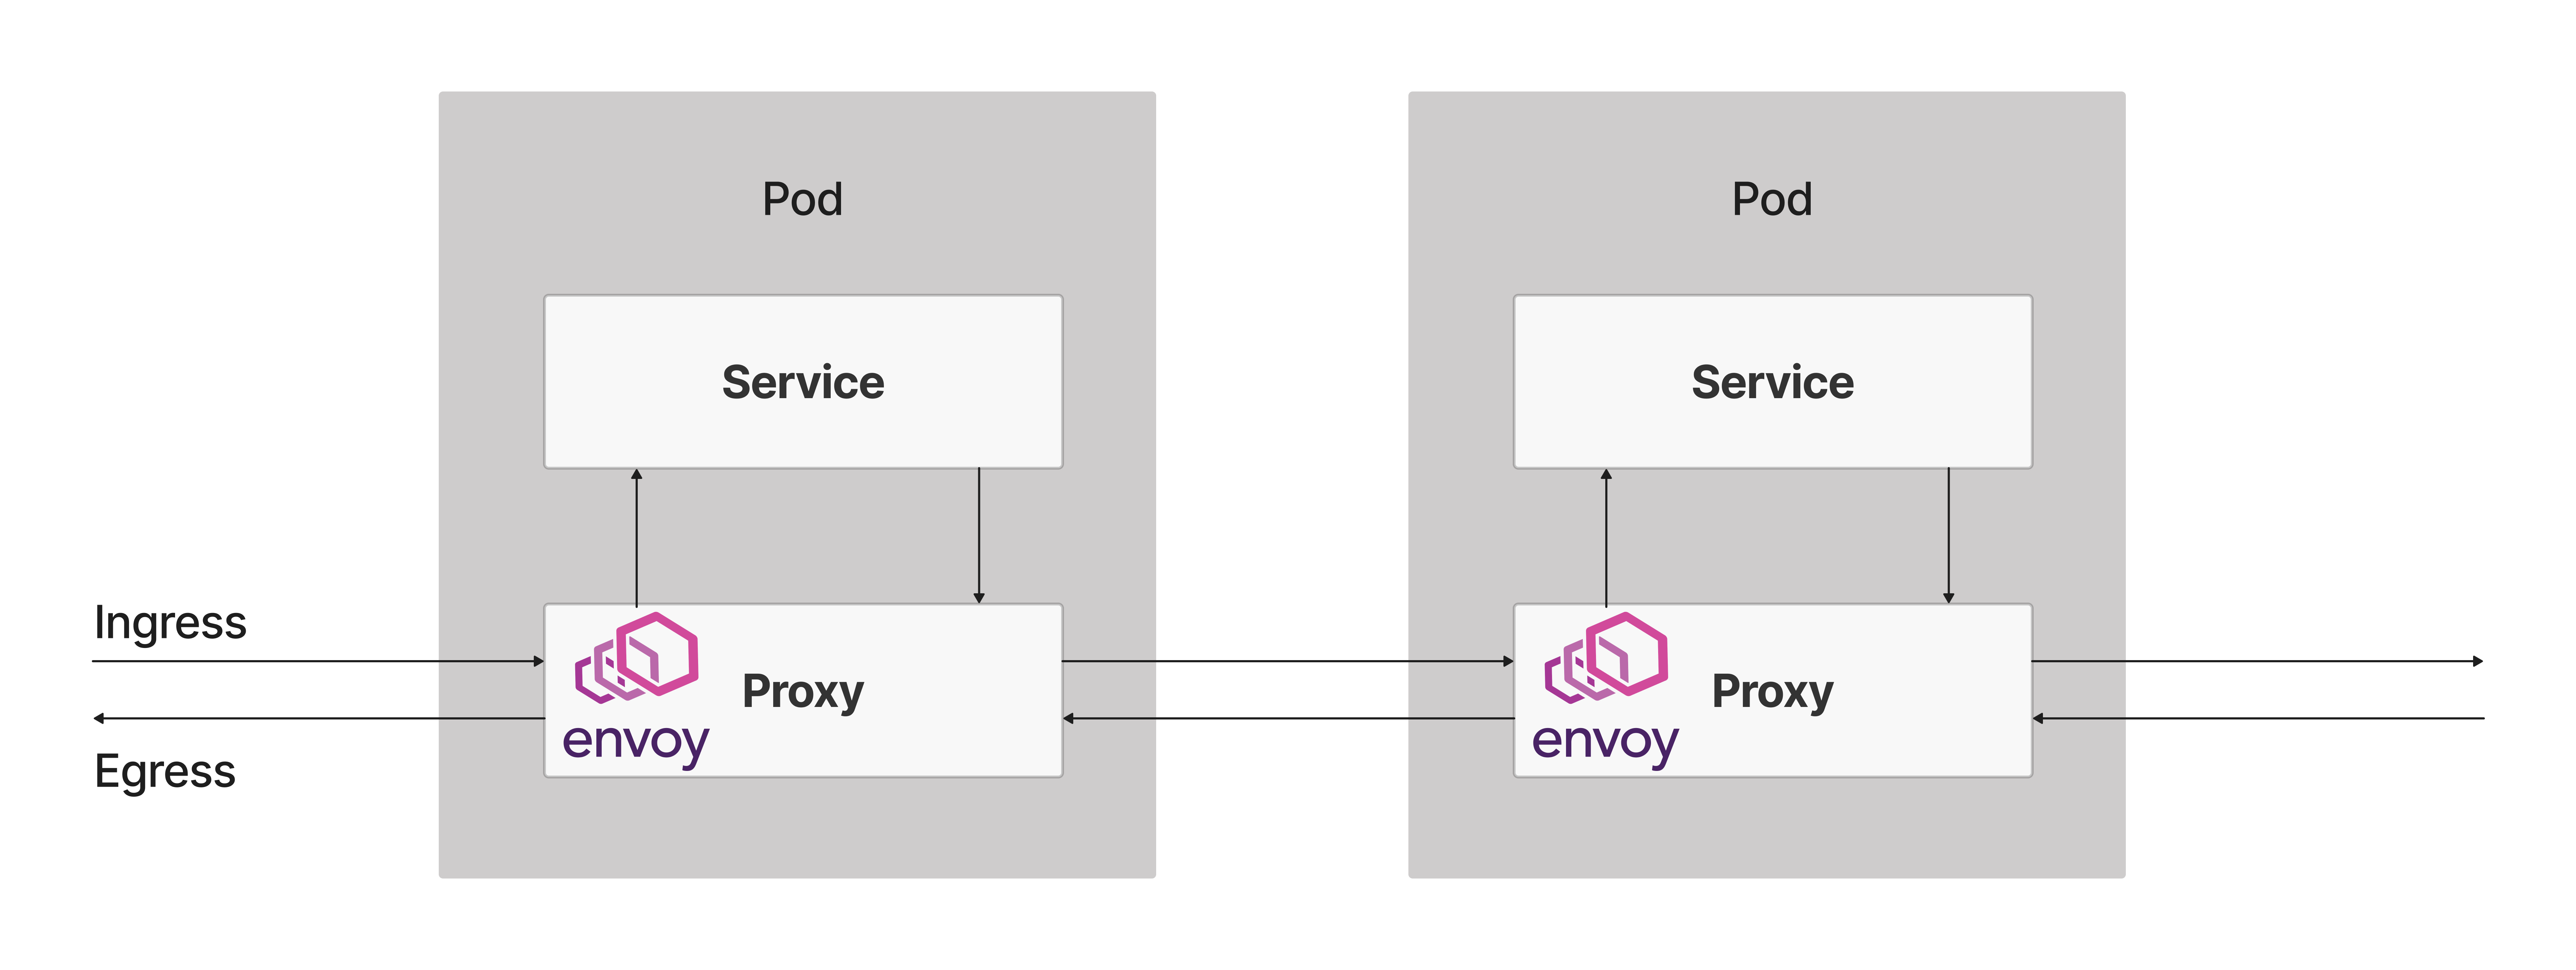
\includegraphics[width=1\textwidth]{assets/diagrams/envoy-proxy.png}
	\caption{Envoy proxy injection and interaction with service inside of a pod.}
	\label{fig:envoy-proxy-injection}
\end{figure}

% \subsection{Locality Load Balancing}
The default load balancer algorithm for Istio is round-robin, where traffic is distributed to clusters in a circular way such that each cluster will be chosen once in a cycle. One of the benefits of this approach is that it prevents an instance where a single server is overloaded by requests by distributing traffic equally to all servers. An approach to reduce latency by closing the physical gap between user and server, locality load balancing is proposed as a better solution for an application with geo-distributed clusters. Locality load balancing is a feature of Istio from using another open-sourced application called Envoy. Locality load balancing, also known as geographical load balancing, is a location-aware load balancer that can efficiently route traffic to the nearest cluster available and can be seen in \autoref{fig:locality-lb-diagram}. To enable locality load balancing, a DestinationRule resource must be configured. DestinationRule defines rules that apply to traffic for a service. DestinationRule can be configured to enable load balancing and outlier detection which work together to determine healthy hosts that are able to handle the traffic.

\begin{figure}
	\centering
	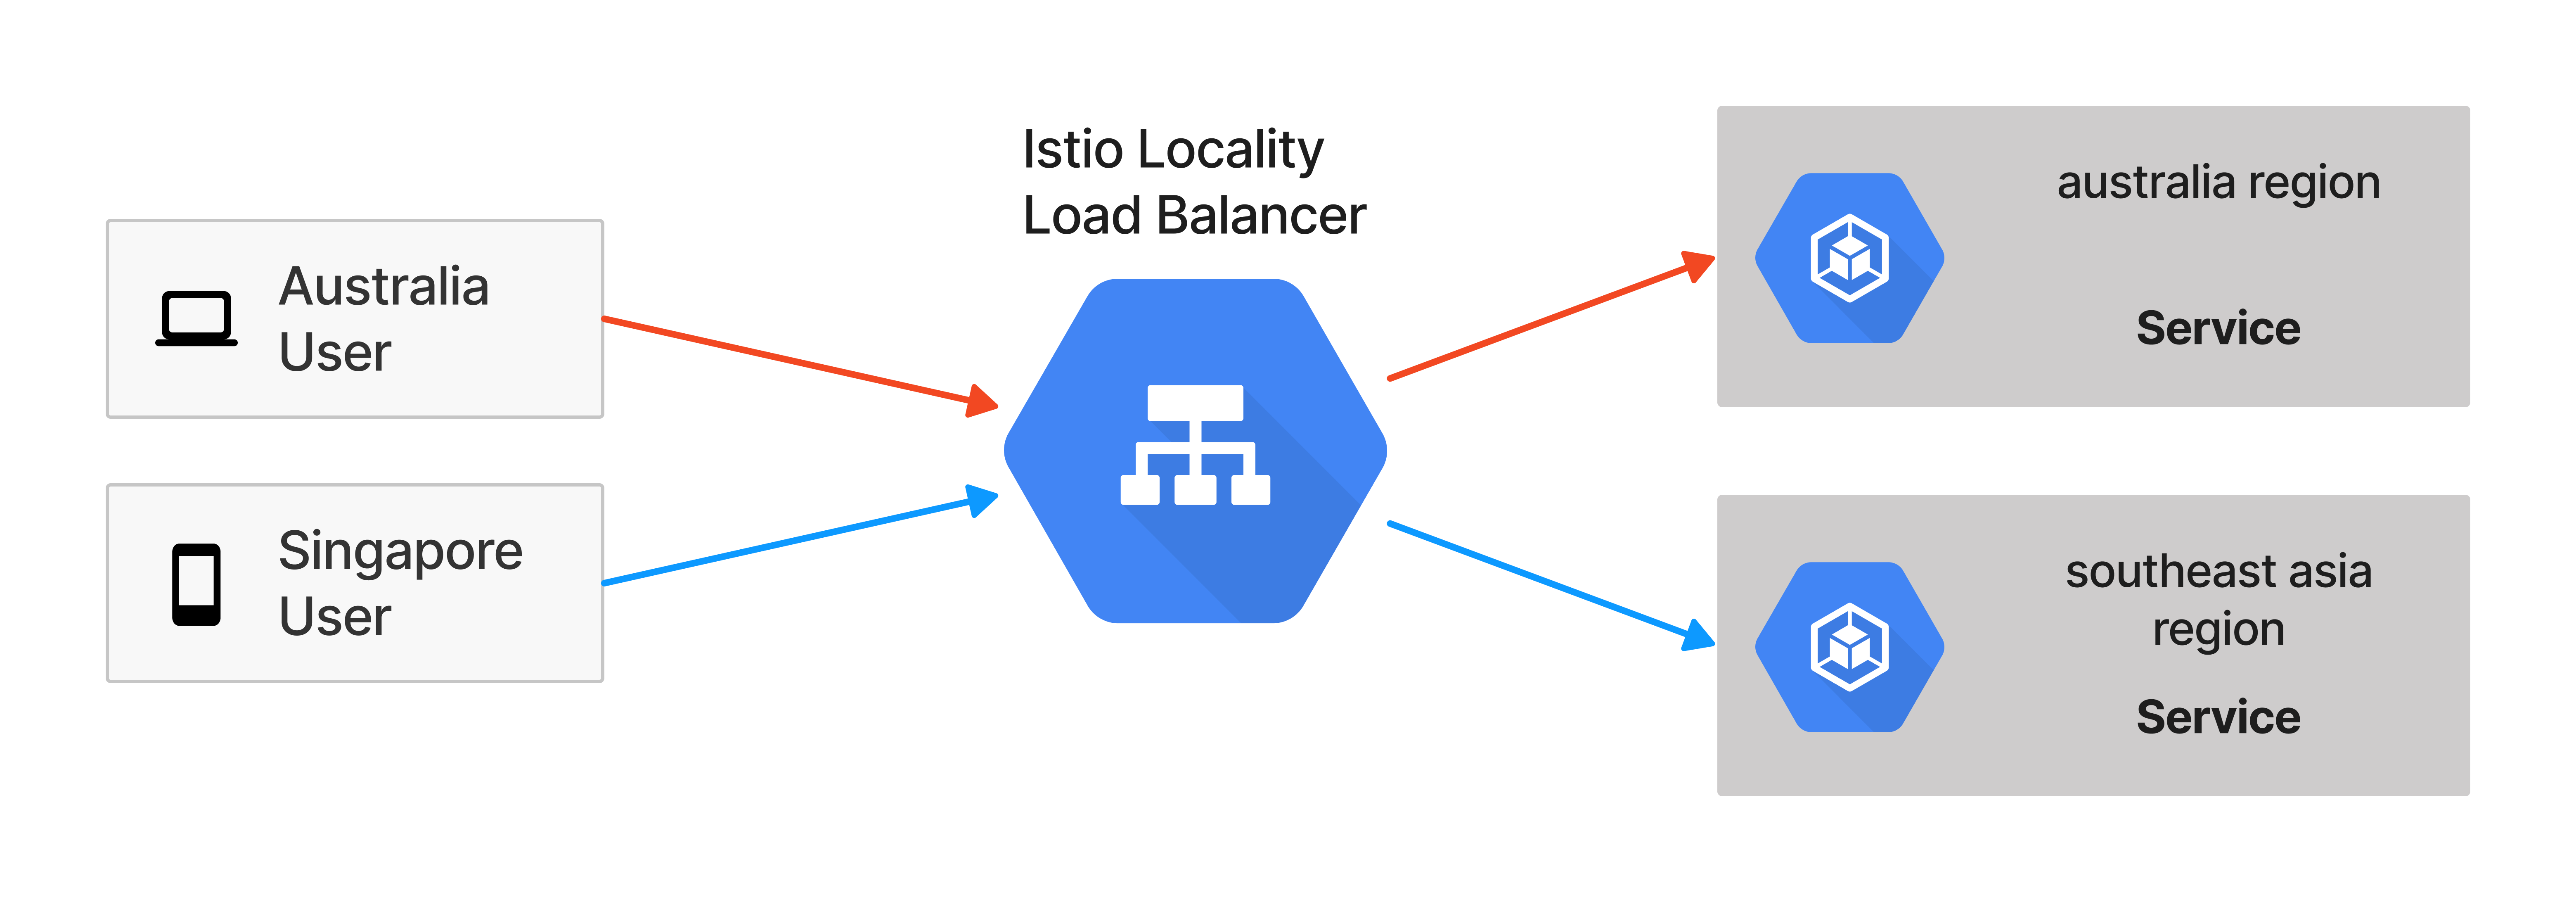
\includegraphics[width=1\textwidth]{assets/diagrams/locality-lb-diagram.png}
	\caption{Istio Locality Load Balancer traffic routing.}
	\label{fig:locality-lb-diagram}
\end{figure}

The main difference between these two methods is their architecture. Istio / ASM introduces an additional layer of complexity, built on top of the Kubernetes architecture to add functionalities that utilize Istio's proxy injection on each pod. Meanwhile, the MCS with MCI approach is an extension of the Kubernetes API, where additional resources such as MultiClusterService and MultiClusterIngress are used to take advantage of Google Cloud's multi-region servers. In addition, MCS with MCI only has a fraction of features compared to Istio / ASM, as it is intended to be used in conjunction with other Google services such as the Google Cloud Load Balancer.

% When we create an Istio ingress, a public IP address is reversed for the dedicated LoadBalancer \citep{xie-2020}.

\section{Performance}
Performance is an important part of web applications and can be measured using different evaluation metrics. The metrics that can measure an application's performance are latency, requests per second, and success rate. Latency is the amount of time it takes for a server to respond to complete a user's request. Lower latency is better, as it results in more requests that are able to be handled and reduces the load of a server. Most importantly, lower latency creates a better user experience as it minimizes the time a user needs to wait while using an application. Latency itself doesn't paint the full picture of application performance, requests per second (RPS) can help measure an application's ability to handle multiple users simultaneously and is a measurement of how many requests an application can handle in a period of time. During peak hours when the application traffic is at its highest, having a high RPS reduces the occurrence of a server bottleneck.

Furthermore, another important metric for a web application to have is reliability. A web service's reliability is the likelihood of a server finishing a request under certain time and workload conditions  \citep{bhalerao-2019}. Measuring a server's reliability is useful to determine how well a server can handle certain real-world scenarios such as high-traffic hours, where a website can expect a heightened number of requests. Without application reliability, businesses that rely on web applications could potentially lose a significant amount of revenue as users aren't able to complete their transactions due to their servers not being able to respond to the client's requests. To measure the percentage of requests being processed as intended, success rate is a metric to quantify just that. Success rate is a measure of how often an application successfully responds to the user's request. A failure can occur when a user inputs something unintended or when a server is unable to process a request caused by the server being overloaded and is indicated by a response code outside of [200, 400], inclusive. The latter definition is used when referring to a failed response as requests are validated and standardized in testing scenarios. 
% It is important for a web application to be reliable, as it could 

To measure the effectiveness of each multi-cluster scenario, performance testing such as load testing and stress testing is done to simulate scenarios where an application receives various amounts of traffic with the possibility of server failure. Load testing is done to measure the performance of a web application at a certain load level to ensure that the website can be worked within the range of multi-user concurrency requirements \citep{yu-2019}. Load testing is also done to identify a server's maximum performance capability by evaluating performance metrics on every increase in load level. On the other hand, stress testing is done to analyze the web application's ability to do failure recovery, which happens after a server is forced to restart due to a server failure. Stress testing can identify a machine's readiness to adopt certain changes that consume resources, such as a service mesh. Performance testing and evaluation metrics are crucial to determine the performance of each approach for geo-distributed clusters.


% \begin{itemize}
%     \item Latency \\
%     Latency is the amount of time it takes for a server to respond to complete a user's request. Lower latency is better, as it results in more requests that are able to be handled and reduces the load of a server. Most importantly, lower latency creates a better user experience as it minimizes the amount of time a user needs to wait while using an application.
%     \item Requests per second \\
%     Requests per second (RPS) is a measurement of how many requests an application can handle in a second. RPS can measure an application's ability to handle multiple users simultaneously. During peak hours when the application traffic is at its highest, having a high RPS reduces the occurrence of a server bottleneck.
%     % \item Survivability \\
%     % Survivability is a measu
%     \item Success rate \\
%     The success rate measures how often an application successfully responds to the user's request. A failure can occur when a user inputs something unintended or when a server is unable to process a request caused by the server being overloaded and is indicated by a 5xx response code. The latter definition is used when referring to a failed response as requests are validated and standardized in testing scenarios. 
% \end{itemize}
